\documentclass{ctexart}
\usepackage{appendix}
\usepackage{listings}%插入代码
\usepackage{xcolor} 
\usepackage{graphicx}%插入表格
\usepackage{booktabs} %绘制表格
\usepackage{caption} %标题
\usepackage{geometry}
\usepackage{array}
\usepackage{amsmath}
\usepackage{amssymb}
\usepackage{subfigure} %插入图片
\usepackage{longtable}
\usepackage{abstract}%摘要
\pagestyle{plain} %页眉消失
\usepackage{setspace}
\usepackage{multirow}%表格
\usepackage{diagbox}
\usepackage{enumerate}%序号
\usepackage{float}%固定图片或表格的位置
\usepackage{gensymb}
\usepackage{microtype}

\def\al{\alpha}
\def\b{\beta}
\def\t{\theta}
\def\c{\circ}
\def\sn{\sum_{i=1}^9}
\def\sm{\sum_{i=1}^{14}}
\def\d{\Delta}
 
\geometry{a4paper,left=2.0cm,right=2.0cm,top=2.0cm,bottom=2.0cm}%页边距
\lstset{
	numbers=left, %设置行号位置
	numberstyle=\tiny, %设置行号大小
	keywordstyle=\color{blue}, %设置关键字颜色
	commentstyle=\color[cmyk]{1,0,1,0}, %设置注释颜色
	escapeinside=``, %逃逸字符(1左面的键),用于显示中文
	breaklines, %自动折行
	extendedchars=false, %解决代码跨页时,章节标题,页眉等汉字不显示的问题
	xleftmargin=1em,xrightmargin=1em, aboveskip=1em, %设置边距
	tabsize=4, %设置tab空格数
	showspaces=false %不显示空格
}
 
\title{基于非线性约束最优化算法的无人机纯方位无源定位模型}
\date{2022/9/18}
 
\begin{document}
	\maketitle
	\renewcommand{\abstractname}{\Large 摘要\\}
	\begin{abstract}
		\normalsize
		本文首先依据无人机圆形编队的几何关系,将接收信号无人机的$\al_1,\al_2$作为参数建立纯方位无源定位模型。
		对编队无人机调整位置进行遍历,并利用暴力算法给出了无人机圆形编队调整方案,并将该定位模型与调整方案向不同的无人机编队进行推广。

		考虑以“发射信号的不同无人机组合”为区别,将问题一中的(1)问题拆分成4种大情况,每个大情况中的2种小情况进行分析。
		首先建立统一的极坐标系,对每一种小情况内的边角关系列出方程组,利用平面几何中的正弦定理、余弦定理以及相关的几何性质对接收信号无人机位置的求解。
		求解后对每一个结果进行合并归类,逐步建立起以无人机之间相对位置为判断条件的,以接受无人机角度信息为参数的纯方位定位模型。答案见方程组(1)(2)(3)。

		并在问题一(2)中采用数学分析原理的相关知识,进一步证明问题(1)中无人机数量的缺陷与不完备性,
		阐述最优的发射信号无人机数量,求出具有完备性的最优发射信号无人机数量选取。求出了还需要2架无人机发射信号,可以实现无人机的有效定位。

		问题一(3)中,对上述问题(1)(2)的结果进行整合,通过无人机纯方位无源定位模型,分析实际圆形编队中的边角关系,依据该理论建立含限制条件的非线性最优化问题。
		结合题目中要求的最终编队状态,使用全搜索算法,逐步逼近直至最终求出最优的调整方案。
		最终的调整总距离$d=52.082630$米。

		问题二中,分析无人机锥形编队的几何关系,对问题一中提出的纯方位无源定位模型进行重构,做出合理的实际假设,建立极坐标系,
		并再次对“发射信号的不同无人机组合”进行分类讨论,同样利用相关定理对接收信号无人机位置进行求解。
		并证明最小发射信号无人机的数量,求出最优的发射信号无人机选取方案。
		并基于搜索算法,同样建立起非线性优化问题,并求解。
		利用解出的结果,设计成无人机的位置调整方案。

		\textbf{关键字}:\bf{暴力遍历算法,非线性最优化,最小二乘法}
	\end{abstract}
	\newpage
	
	\section{问题的重述}
	无人机集群在遂行编队飞行时,为保持编队队形,采用纯方位无源定位的方法调整无人机的位置,
建立精度高,速度快的数学模型以确定并调整无人机位置是一个重要课题。
\par
问题 1
10 架无人机组成的圆形编队,其中 9 架无人机(编号 $F1$~$F9$)均
匀分布在某一圆周上,另 1 架无人机(编号 $F0$)位于圆心。无人机均保持在同一高度上飞行。
\par
	(1) 位于圆心的无人机($F0$)和编队中另 2 架无人机发射信号,其余位置有偏差的无
人机被动接收信号。当发射信号的无人机位置无偏差且编号已知时,建立被动接收信号无人机
的定位模型。
\par
	(2) 某位置略有偏差的无人机接收到编号为 $F0$ 和 $F1$ 的无人机发射的信号,另接收到
编队中若干编号未知的无人机发射的信号。若发射信号的无人机位置无偏差,除 $F0$ 和 $F1$
外,还需要几架无人机发射信号,才能实现无人机的有效定位?
\par
	(3) 按编队要求,1 架无人机位于圆心,另 9 架无人机均匀分布在半径为 100 m 的圆周上。
当初始时刻无人机的位置略有偏差时,请给出合理的无人机位置调整方案,即通过多次调整,
每次选择编号为 $F0$ 的无人机和圆周上最多 3 架无人机遂行发射信号,其余无人机根据接收
到的方向信息,调整到理想位置(每次调整的时间忽略不计),使得 9 架无人机最终均匀分布在
某个圆周上。利用给出的数据,仅根据接收到的方向信息来调整无人机的位置,请给出具
体的调整方案。
\par
\vspace{0.5em}
	问题 2 实际飞行中,无人机集群也可以是其他编队队形,例如锥形编队队形(直
线上相邻两架无人机的间距相等,如 50 m)。仍考虑纯方位无源定位的情形,设计无人机位置
调整方案。
	\section{模型假设}
\begin{enumerate}
	\item 假设所有无人机所处的外界环境保持稳定且适宜无人机进行飞行动作。
	\item 假设所有无人机不受外界电磁干扰,各无人机接收与发射的信号无失真。
	\item 假设所有无人机始终保持在同一高度上飞行。
	\item 假设各无人机之间互不影响,调整位置时准确且无误,并忽略调整的时间。
	
	
	\end{enumerate}
	\section{符号说明}
	\begin{center}
		\setlength{\tabcolsep}{9mm}{
			\begin{tabular}{ccc}
				
				
				\toprule  %添加表格头部粗线。
				\textbf{符号} & \textbf{意义} & \textbf{单位}\\
				\midrule  %添加表格中横线
				$\alpha_1$ & 接受的角度信息1 & 弧度($rad$)\\
				$\alpha_2$ & 接受的角度信息2 & 弧度($rad$)\\
				$\al_3$ & 接受的角度信息3 & 弧度($rad$)\\
 				$\beta$    & 发射信号无人机的角坐标 &弧度($rad$)\\
				$\rho$ & 发射信号无人机的距离坐标 &米($m$)\\
				$r$ & 圆的半径 & 米($m$)\\
				$F0\sim F15$ & 对应各个无人机的名称 & \\
				$n$ & 发射机之间的距离单位 & 个\\
				$d$ & 调整无人机的距离和 & 米($m$)\\
				\bottomrule %添加表格底部粗线
		\end{tabular}}
	\end{center}
	注:$\alpha_1$与$\alpha_2$的取法为以接收信号的无人机为圆心的逆时针方向分别取为$\alpha_1$,$\alpha_2$,且$\al_3=\al_1+\al_2$。
	$\beta$的取法为发射无人机与正半轴所成的优角(小于$180^\circ $)。发射机表示发射信号的无人机,接收机表示接受信号的无人机。
	
	\section{问题分析}
	
	\subsection{问题一分析}
	问题一中包含了三个小问,实质上讨论的都是建立在被动接受信号无人机的定位模型之上。
	\par 问题一(1)旨在建立被动接受信号无人机的定位模型,当已知角度信息$\alpha_1$,$\alpha_2$和$\alpha_3$
	时通过在无人机$K0$处建立以$K0$到$K1$方向为正方向的极坐标系,对一共4种发射信号的无人机相对位置进行分类讨论,
	使用包括接收机在内的一共4个无人机的几何关系建立一系列方程组,使用正弦定理与余弦定理求解出其余略有偏差的无人机的位置信息。
	
	\par 问题一(2)需要确定额外无人机的数量,利用问题(1)中求解出的定位模型,证明出仅选取3架无人机发射信号的不完备性,即存在无法涵盖的无人机位置。
	求出不同数量无人机发射信号时的有效性,从而解出最好的无人机选取方法。

	\par 问题一(3)则在前两问基础上再进一步考虑调整的方案,使用表格中给出的位置数据,使用设计的调整算法使得
	经过多次调整后9架无人机处于$K0$为圆心,100m为半径得圆周上。最优的调整方案应满足总调整次数较少,单次调整幅度较低,
	最终位置误差较小。将问题(3)转化成非线性最优化问题,或采用随机搜索的数值逼近方法,
	利用接受到的$\alpha_1$,$\alpha_2$和$\alpha_3$角度信息确定最优位置,对其余无人机进行调整,使最终结果靠近理想状态。

	\subsection{问题二分析}
	问题二中需要建立面对锥形编队队形的纯方位无源定位模型,总体的建立与调整方案与问题一中圆形编队模型类似,同样需要建立
	坐标系,求解处各个无人机的理想位置信息,并且计算出无人机的实际位置信息,使整个锥形编队处于理想的编队队形。

	\newpage
	\section{问题一模型建立与求解}
	\subsection{问题(1)模型的建立与求解}
	\subsubsection{问题(1)模型的建立}

	本题中需要以接受信号的$\alpha_1$,$\alpha_2$和$\alpha_3$角度信息对被观测无人机的位置进行求解,可以不失一般性的
	建立以$F0$无人机为原点,$F0$指向$F1$的方向为正半轴的极坐标系。该圆的半径不妨设为$r$。
	经过分析可知,该定位模型的建立应以几何学为基础,只需给定$\alpha_1$,$\alpha_2$和$\alpha_3$的角度信息
	最终得出被测无人机的相关位置信息。
	并通过分析可得在圆周上选取的2架无人机会存在4种情况。
	分别是两架无人机间间隔为0(架)、间隔为1、间隔为2、间隔为3。这是因为理想状态下9架无人机组成正九边形,由几何关系可知
	间隔为4的情形可以转换为间隔为3的情况(见图1)。图中4种不同颜色的连线表征为圆周不同无人机的组合,因此$F1$与$F6$的组合
	可以相似的转换为间隔为3的$F1$与$F5$组合。
	
	\begin{figure}[htbp]  %插入图片
		\centering
		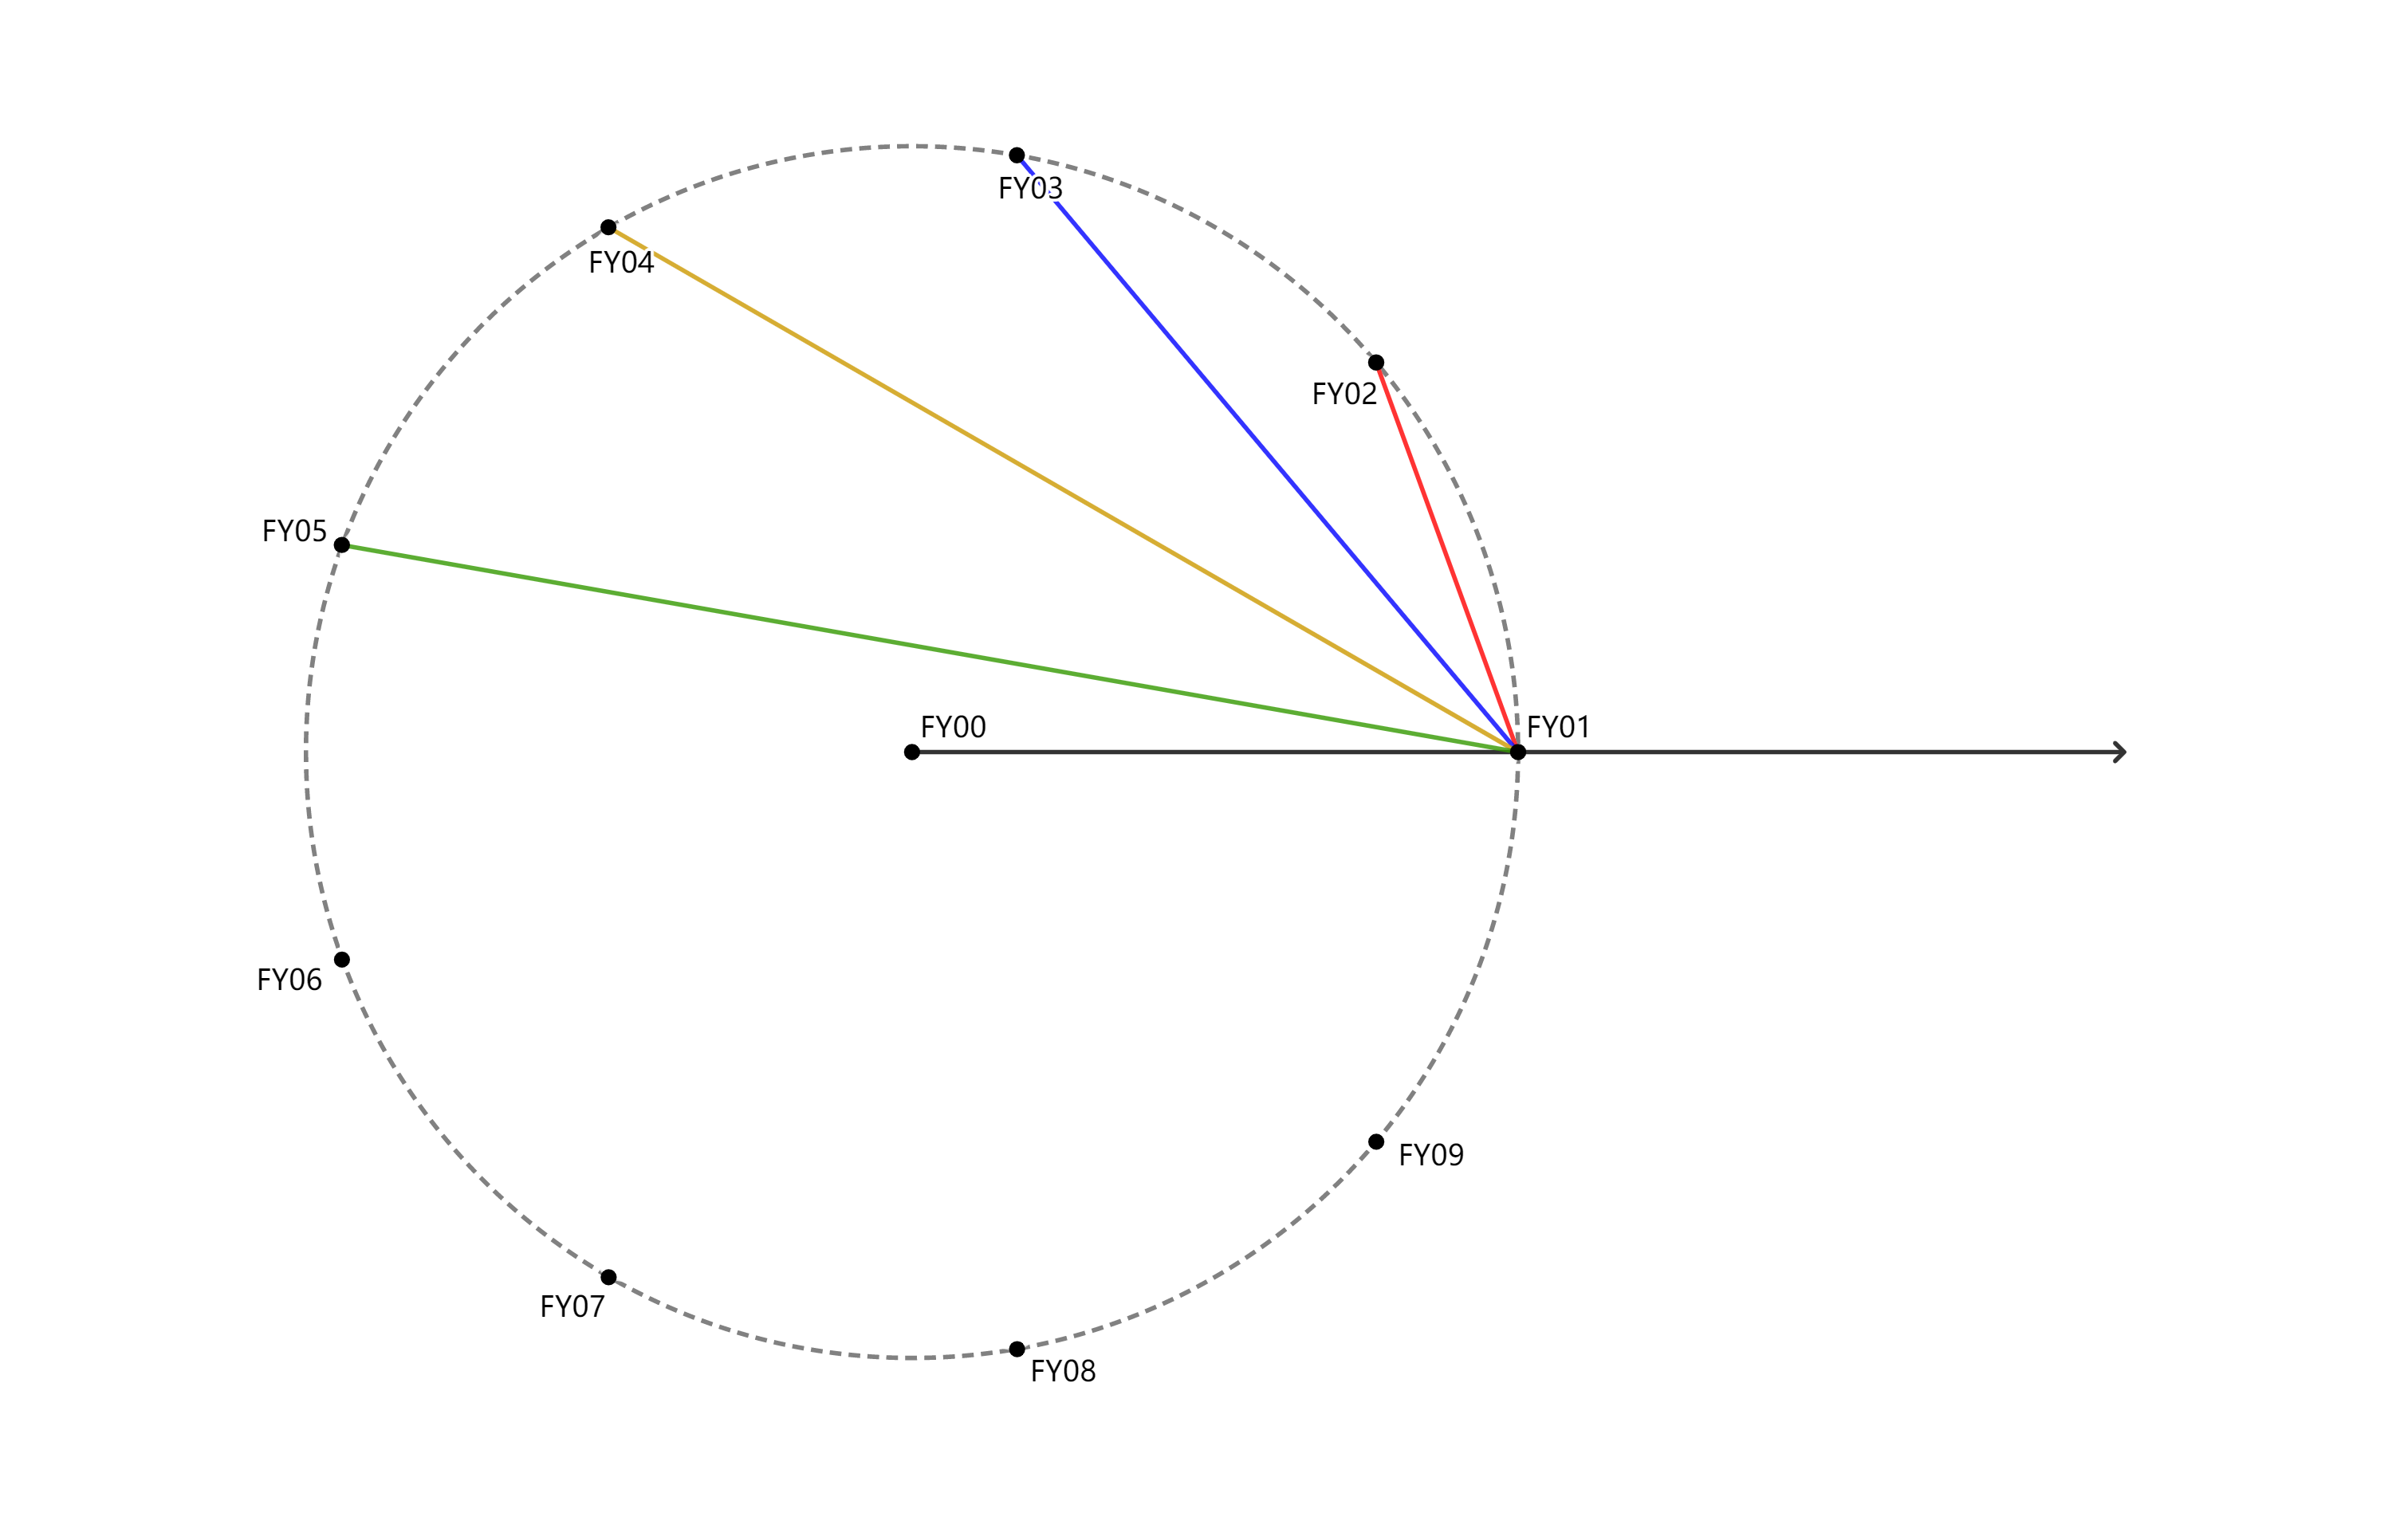
\includegraphics[scale=0.6]{pic/1.png}
		\caption*{图1}
		\label{fig1}
	\end{figure}

	\par
	选取$F1$与$F2$时不存在向无人机之间发射信号的情况,间隔为1、2、3时均有可能向无人机之间发射信号的可能。
	例如$F1$,$F3$以及$F0$共同向$F2$发射信号,此时所产生的三角形角度关系则截然不同。
	因此更深入地讲,可以将选取$F1$与$F2$归为一类,因为只有可能向外即$F3,F4,F5,F6,F7,F8,F9$发射信号,
	将其余地归为一类。
	
	\subsubsection{问题一(1)模型的求解}
	\noindent $(i)$下面将举例求解以$F0$、$F1$、$F2$组合发射信号,对其余无人机求解的方法。
	\par
	已知$\alpha_1$,$\alpha_2$,并且 $F1(r,0)$, $F2(r,\beta)$。
	利用余弦定理即可求解出角 $a$的表达式,即可求解出接受信号的无人机$F8'$的极坐标(见图2)。
	由几何关系可列出一下方程组:($\angle F2F1F8$简写为$F218$)

	\[\left\{
    \begin{aligned}
    &\frac{r}{\sin \angle F2 1 8}=\frac{l}{\sin \angle F208}\\
    &\angle F218+\angle F208 +\al_1 +\al_2 +\frac{\pi -\b}{2} = 2\pi\\
	&l=2r\cdot \sin(\frac{\b}{2})
    \end{aligned}.
    \right.
	\]

	求解过程中先得
	\begin{equation*}
		\angle F218= \frac{3\pi}{2}+\frac{\b}{2}-(\angle F208 +\al_1 +\al_2 )
	\end{equation*}

	左右同取sin函数,利用sin函数的和角公式,则
	\begin{equation}
		\sin \angle F218 = \cos(\frac{\b}{2}-\al_1-\al_2- \angle F208)\tag{*}
	\end{equation}

	将两角的关系等式
	\begin{align*}
		\frac{r}{\sin \angle F2 1 8}=\frac{l}{\sin \angle F208},\;\;\mbox{将之代入(*)}
	\end{align*}

	我们可以得到$\tan\al_2$相应的数值。
	最终的结果为 $F8'( \rho, \theta )$.
	其中
	\begin{equation}
		\begin{aligned}
			&\t=\arctan( \frac{\cos\b \cdot \tan\al_2-\sin\b}{1-\cos\b-\sin\b \cdot \tan\al_2}  )\\
			&\rho=\frac{r}{\sin(\alpha_1 + \alpha_2)}\cdot \sin(\alpha_1+\alpha_2+\theta)\\
			&\b=40^\c
		\end{aligned}
	\end{equation}

	% \begin{align*}
	% 	&\theta=-\arctan(\frac{\cos(\alpha_1 + \alpha_2-\frac{\beta}{2})}{\sin(\alpha_1 + \alpha_2-\frac{\beta}{2}) - \frac{\sin(\alpha_1)}{2\sin(\alpha_2)\sin(\frac{\beta}{2})}})-\beta\\
	% 	&\rho=\frac{r}{\sin(\alpha_2)}\cdot \sin(\b+\t+\alpha_2)\\
	% 	&\b=40^\c
	% \end{align*}

	\begin{figure}[htbp]  %插入图片
		\centering
		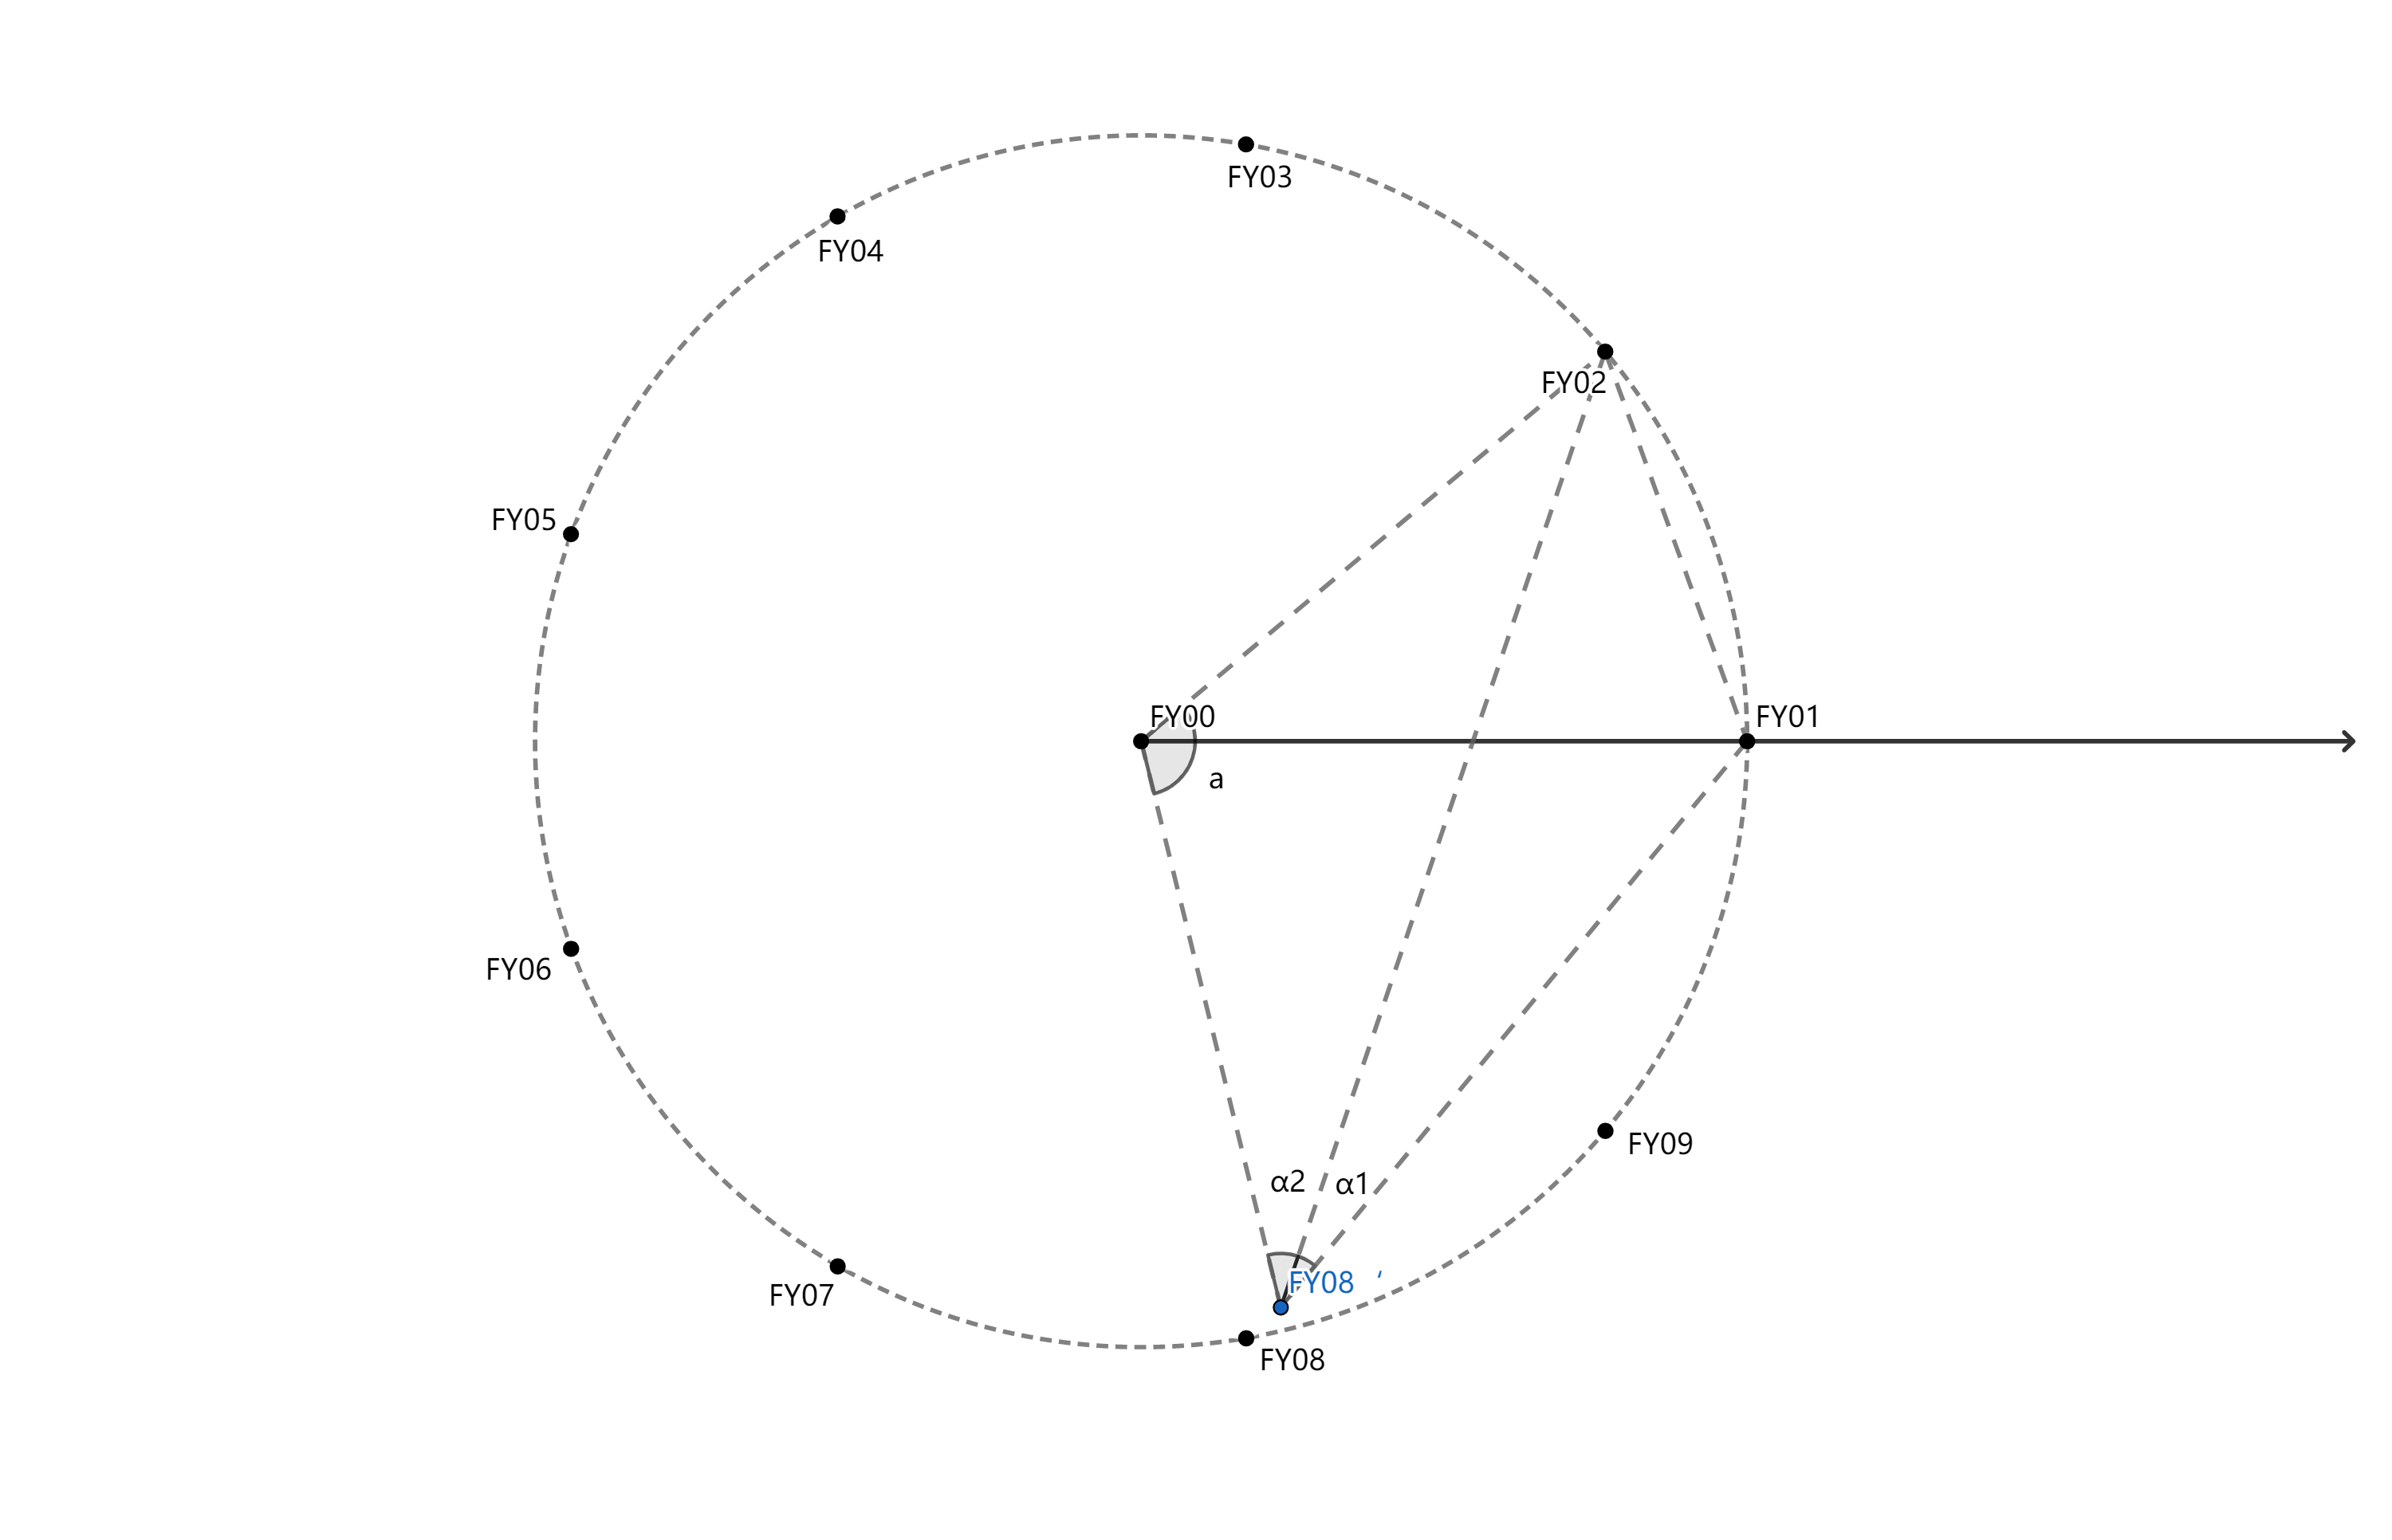
\includegraphics[scale=0.6]{pic/2.png}
		\caption*{图2}
		\label{fig2}
	\end{figure}

\vspace{0.5em}	
	$(ii)$下面将求解$F1$分别与$F3,F4,F5$组合发射信号的清形。
	\par
	当向外发射信号时,例如$F1,F4$确定$F8'$的位置时,此时$\beta$角为钝角(见图3),最终可以求解得
\begin{equation}
	\begin{aligned}
		&\t=\arctan( \frac{\cos\b \cdot \tan\al_2-\sin\b}{1-\cos\b-\sin\b \cdot \tan\al_2}  )\\
		&\rho=\frac{r}{\sin(\alpha_1 + \alpha_2)}\cdot \sin(\alpha_1+\alpha_2+\theta)\\
		&\b=n\cdot 40^\c,  \;\;\;\;n\in\{2,3,4\}
	\end{aligned}
\end{equation}

\vspace{1em}
	当向内发射信号时,例如$F1,F4$确定$F3'$的位置时,此时$\t$处于角$\b$的内部(见图4),最终可以求解得

\begin{equation}
	\begin{aligned}
		&\t = \arctan ( \frac{\sin\b+\cos\b\cdot \tan\al_1}{1-\cos\b-\sin\b\cdot \tan\al_1} )\\
		&\rho= \frac{r}{\sin\al_2}\cdot \sin(\al_2 +\t)\\
		&\b=n\cdot 40^\c,  \;\;\;\;n\in\{2,3,4\}
	\end{aligned}
\end{equation}

\begin{figure}[htbp]
	\centering
	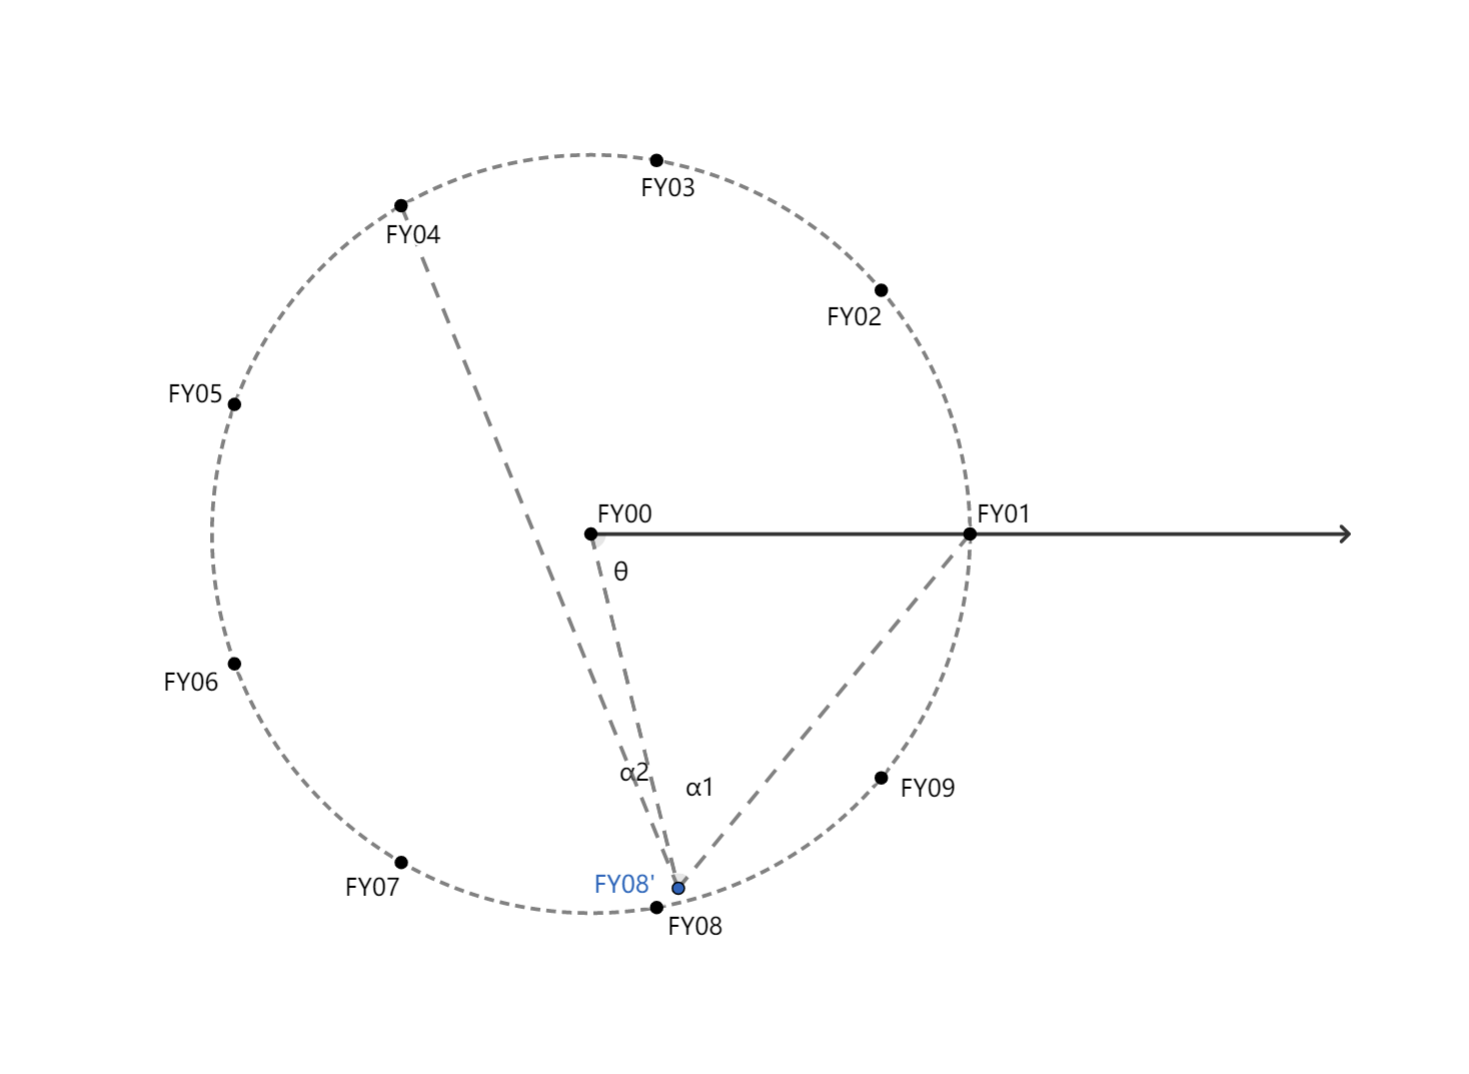
\includegraphics[scale=0.4]{pic/3.jpg}
	\caption*{图3}
\end{figure}

\begin{figure}[htbp]
	\centering
	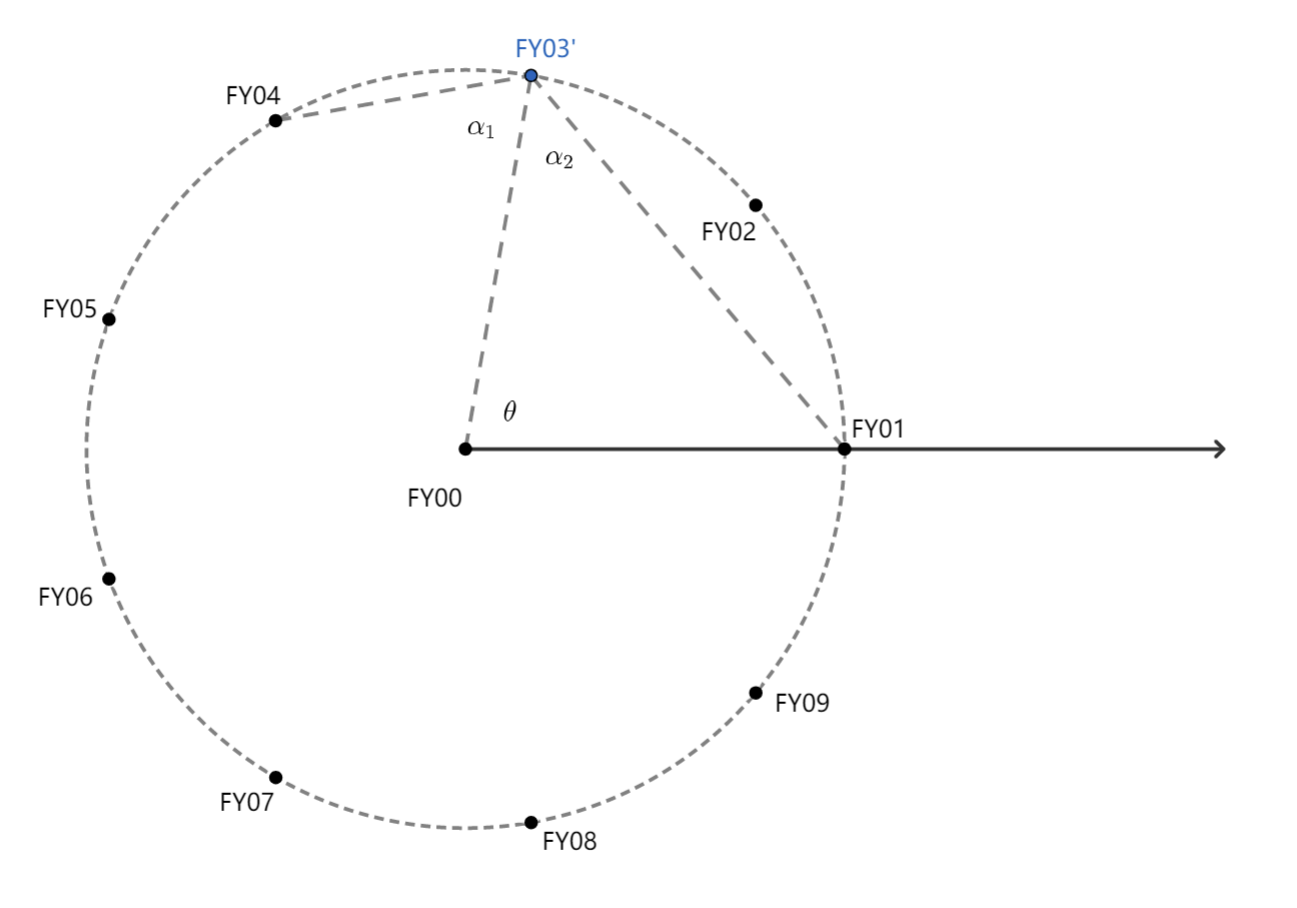
\includegraphics[scale=0.4]{pic/4.jpg}
	\caption*{图4}
\end{figure}

	\par求解中的等式组(1)(2)(3)为不同情况下的三种位置信息转换方程,利用这三种方程组,就可以利用接收到的$\al_1,\al_2,\al_3$三种信息计算出接收机
	的极坐标位置信息,从而实现了纯方位无人机的的定位。

	\vspace{0.5em}
	\subsection{问题(2)的求解:完备的无人机选取}
	此问题中需要选取圆周上几架无人机可以利用问题(1)中建立的定位模型,定位出其余位置略有偏差的无人机的位置。
	例如当选取$F0,F1,F2$无人机发射信号时,可能无法使用问题(1)中求解出的方程组(1)的位置通式得出$F6$无人机的位置。
	此时则需要额外的无人机发射信号,利用新产生的$\al_1,\al_2,\al_3$信息求解。

	在问题(1)中,分情况解出了通解的符号式子。在增加圆周上1架无人机发射信号时,
	观察可知,当$\t$不存在,即$1-\cos\b -\sin\b \cdot \tan\al_2 $为0使得$\arctan$的
	值不存在。在这种情况下可以算出
	\begin{align*}
		\al_2=\frac{\b}{2}+k\cdot \pi, \;\; k\in\mathbb{Z}  
	\end{align*}

	\par
	在圆周选取两架,共4种不同的无人机选取方案下,由于$\t$与除$F1$外另一架无人机的选取有关,
	则$\t$为一个定值,可知接收机所接收的角度信号$2\al_2=\b$的可能性存在,并大概率出现在无人机$F0$处于另外两架中间的情形下。
	因为$\t$无法得出,从而导致了无人机定位失败,此时必然需要一架额外的无人机发射信号以保证定位成功。

	如下图5:

	\begin{figure}[htbp]
		\centering
		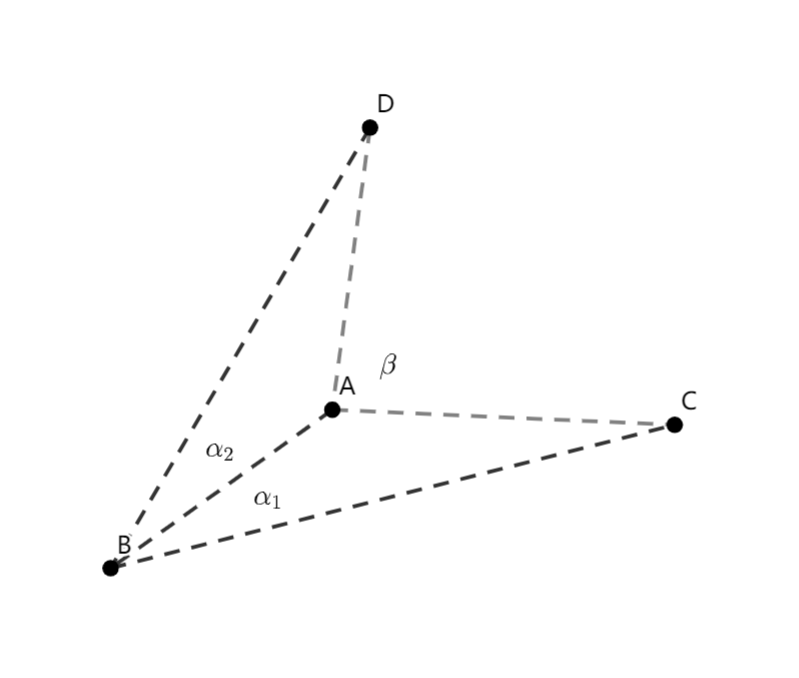
\includegraphics[scale=0.45]{pic/5.png}
		\caption*{图5}
	\end{figure}

	图中的$\al_2=\frac{\b}{2}$可能发生,就会导致点B的角坐标无法求解,也就是B的定位失败。

	\vspace{0.5em}
	接下来考虑添加一架圆周上的无人机发射信号能否将所有可能性包含在内并可解以定位其余无人机。
	利用反证法,证明除$FY00与FY01$外只需增加2个无人机发射信号,即可实现无人机的准确定位。
	\par
	假设增加2个无人机发射信号仍然会存在无法解出其余位置的情况。
	当在圆周上任取三架无人机时,其中有三组发射的组合,
	无法解出其余位置则说明选取后的三种发射组合每一种都存在$\al_2=\frac{\b}{2}$。
	假设其中一组的角度信息为$\al_1,\al_2$,另一组为$\al_1',\al_2'$,
	并定义对应的$\b$与$\b'$(如图6)。例如:

	\begin{align*}
		&\b = \angle F102 ,\;\b' = \angle F104\\
		&\al_1=\angle F170 ,\;\al_2=\angle F470\\
		&\al_1'=\angle F270, \; \al_2'=\angle F470\\
		&\;\;\;\;\;\;\;\;\;\;\;\;\;\;\al_2=\al_2'.
	\end{align*}

	\begin{figure}[htbp]
		\centering
		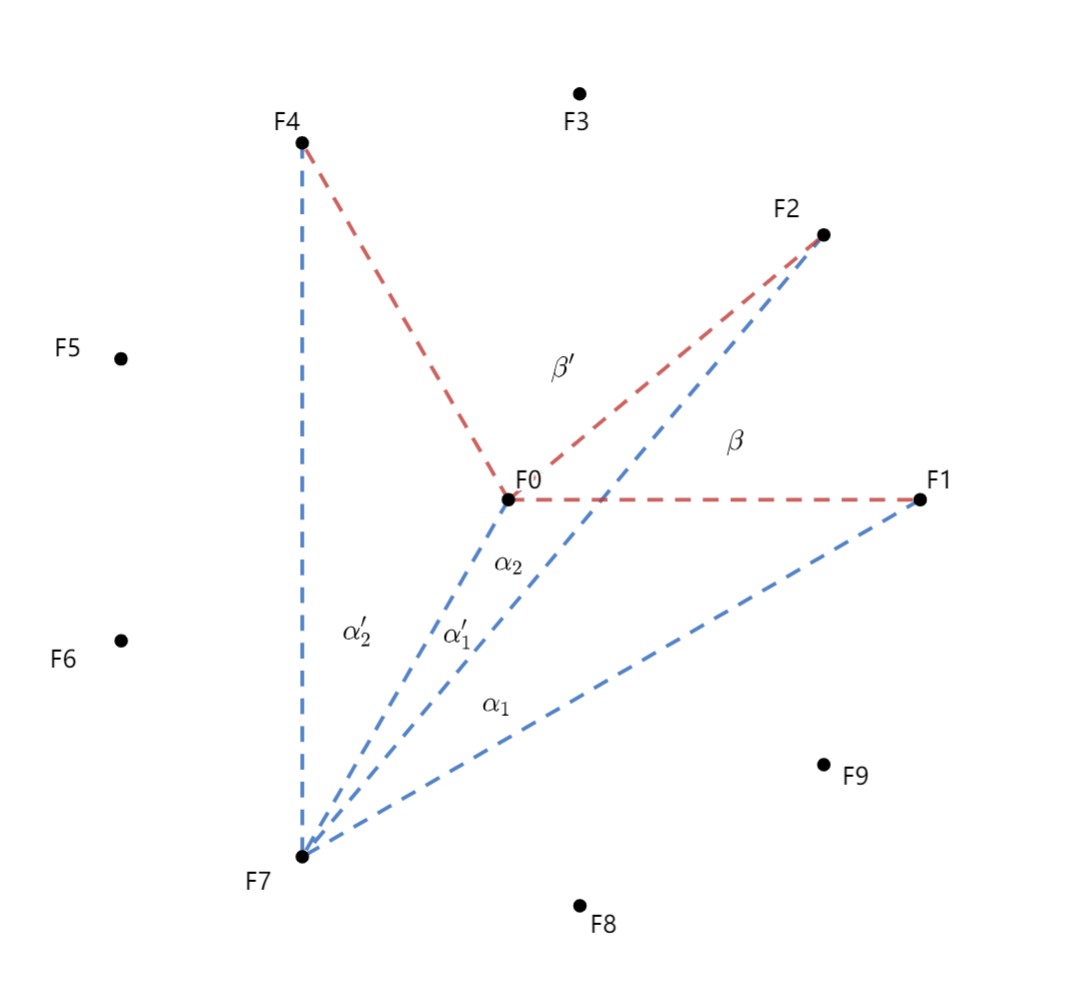
\includegraphics[scale=0.45]{pic/6.png}
		\caption*{图6}
	\end{figure}

	\newpage
	按照假设,则有
	
	\[\left\{
    \begin{aligned}
		&\al_2=\b\\
		&\al_2'=\b'\\
		&\al_2=\al_2'
    \end{aligned}.
    \right.
	\]

	根据图6,两种组合其中有一个角度信息重合,$\al_1'=\al_2$。
	\par
	因上述方程组不可能成立,与证明假设同时成立相互矛盾,
	因此假设不成立,即
	\begin{align*}
		\al_2\neq \frac{\b}{2}, \;\; \forall \mbox{不同发射组合所生成的$\al_1,\;\al_2$信息}.
	\end{align*}
	\par 即增加2个无人机发射信号不会存在无法解出其余位置信息的情况,
	即任意增加2个无人机发射信号可以对其余所有无人机位置进行求解。

	\par下面考虑额外选取数量超过2的情况。例如额外选取$F2,F3,F4$进行信号的发射,此时一共由6种不同的信号发射组合,其中包含了上述所考虑的三种。
	(额外选取$F2,F3$时的三种组合)
	而在之前的证明中,证明了额外选取$F2,F3$时可以实现其余无人机的定位。
	更进一步,选取2架的方案比选取3架的方案少发射了3组信号,可以使用资源更少,而达到相同的目标,所以选取2架的方案更优。
	同理选取2架的方案比选取更多无人机的方案更优。
	
	\par所以问题(2)中还需要两架无人机发射信号,以达到无人机有效定位的实现。
	
	\newpage
	\subsection{问题(3)的求解}
	本问题中,不仅需要利用(1)(2)中构建的无源定位模型对所有无人机进行位置的确定,还需要更进一步确定定位后的调整方案,使最终总体的调整难度要较低。

	\par
	利用geogebra描绘初始状态的无人机编队位置如下图7:(蓝色为无人机)

	\begin{figure}[htbp]
		\centering
		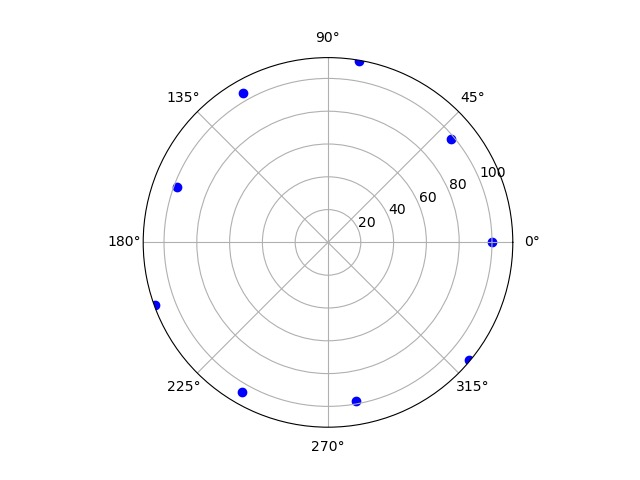
\includegraphics[scale=0.35]{pic/7.jpg}
		\caption*{图7}
	\end{figure}

	首先依据题目(1)相同地,建立极坐标系。
	根据题目所要求可知,调整后最终需要所有无人机均匀地分布在半径为100m的圆周上。
	即所有相邻无人机之间间隔40度,所有无人机距离圆心无人机距离为100m。
	而分析题目中表1所给出的数据发现,无人机$FY00,FY01$的相对位置正确,距离为100m,也就是说该圆周已确定。
	因此当无人机$FY00,FY01$确定时,所有无人机的理想位置均已知,移动无人机$FY01$就会连锁地导致其余无人机的理想位置发生变化。
	所以本题对无人机位置调整方案的求解可以转化为在一系列限制条件下,对无人机$FY01$位置的求解。
	因此在一定的限制条件下,列出非线性的约束方程组,使用暴力算法求解出目标函数即$FY01$的最优位置,再将其余无人机沿直线移动到最优位置上即可。
	
	\par在求解问题(1)时,可知所有无人机的极坐标位置信息均可由所接收到的位置信息即$\al_1,\al_2,\al_3$求解得出,
	因此各个无人机的移动前后的极坐标均可通过不同的角度信号求出。
	另最终编队状态唯一,为所有无人机均匀地分布在半径为100m的圆周上,不会产生无人机位置偏差的情况。
	所以目标函数可以设置为求所有无人机调整时所飞行的距离和的最小值,即

	\begin{align*}
		min \;\;\; d=\sn \sqrt{r^2 +\rho_i ^2 -2r\rho_i \cdot \cos\d\t_i }
	\end{align*}

	\par
	因为最终编队的相对位置确定,即每个相邻的无人机之间与圆心无人机连线做组成的圆心角固定为$40^\circ$,
	且最终的理想状态下各个无人机距离圆心无人机$FY00$的距离为100m。
	定义$\t_i$为无人机编号为$FY0i$本身位置的角坐标,$\Delta\t_i$为某一无人机调整前后位置与圆心无人机连线所成的角度,
	同时定义$\t_i'$为调整后,理想编队状态下的无人机角坐标,$\rho$为无人机调整前到$F0$的距离,$\rho'$为调整后到$F0$的距离。
	则上述的文字可表述为
	
	\begin{align*}
		&\rho' = 100m\\
		&\t_{i+1}'-\t_{i}'=40^\circ\\
		&\t_i' = \t_i + \Delta\t_i,\;\; i \in \{1,2,3,4,5,6,7,8\}\\
		&\t_9-\t_1=40^\circ \\
		&\t_9' = \t_9 + \Delta\t_9
	\end{align*}

	则该优化问题可表示为

	\begin{align*}
		Minimise \;\;\;\; &d=\sn \sqrt{r^2 +\rho_i ^2 -2r\rho_i \cdot \cos\d\t_i }\\
		s.t \;\;\;\;&\rho' = 100m\\
		&\t_{i+1}'-\t_{i}'=40^\circ\\
		&\t_i' = \t_i + \Delta\t_i,\;\; i \in \{1,2,3,4,5,6,7,8\}\\
		&\t_9-\t_1=40^\circ \\
		&\t_9' = \t_9 + \Delta\t_9
	\end{align*}

	其中,限制条件可表示为
	\begin{align*}
		A\Delta\t=b
	\end{align*}
	其中
	\begin{align*}
		&A=\begin{pmatrix}
			-1 & 0&0&0&0&0&0&0&1\\
			1&-1&0&0&0&0&0&0&0\\
			0&1&-1&0&0&0&0&0&0\\
			0&0&1&-1&0&0&0&0&0\\
			0&0&0&1&-1&0&0&0&0\\
			0&0&0&0&1&-1&0&0&0\\
			0&0&0&0&0&1&-1&0&0\\
			0&0&0&0&0&0&1&-1&0\\
			0&0&0&0&0&0&0&1&-1
		\end{pmatrix},b=\begin{pmatrix}
				\t_{i+1}-\t_i-40^\circ\\
				\vdots
					\end{pmatrix}
	\end{align*}

	将该优化问题利用MATLAB中的optimization工具包求解,最后求解出结果。

	每个无人机移动的信息如下表:


\begin{center}
	\begin{tabular}{|c|c|c|}
		\hline
		\mbox{无人机编号}&\mbox{$\t_i$的移动角度/度}&\mbox{移动距离/米}\\
		\hline
		FY01&2.81247324225734e-07&0\\
		\hline
		FY02&-0.0999997187526758&2.00744921022749\\
		\hline
		FY03&-0.209999718752676&12.0062673660278\\
		\hline
		FY04&0.250000281247324&5.01995072827991\\
		\hline
		FY05&0.140000281247324&2.01457467470591\\
		\hline
		FY06&0.0400002812473243&12.0002274487071\\
		\hline
		FY07&-0.0699997187526758&5.00156699828755\\
		\hline
		FY08&-0.169999718752676&2.02145328832454\\
		\hline
		FY09&-0.279999718752676&12.0111397208718\\
		\hline
	\end{tabular}
\end{center}
	表中正的$\t_i$的移动角度,为逆时针调整$FY0i$的位置,负数则相反。

\vspace{0.5em}
	最终求解出的总移动距离约为$d=52.082630$米。

\newpage
\section{问题二模型的建立与求解}
	\subsection{问题二模型的建立}
	本题目将题目一中的圆形编队拓展为锥形编队,在保持高度不变的情况下,首先可以建立极坐标系。
	建系时以无人机FY15为直角坐标系原点坐标为(0,0),以初始编队状态下的F15 与F11 连线,
	垂直该连线方向确定极坐标正半轴(如图8)。

	\begin{figure}[htbp]
		\centering
		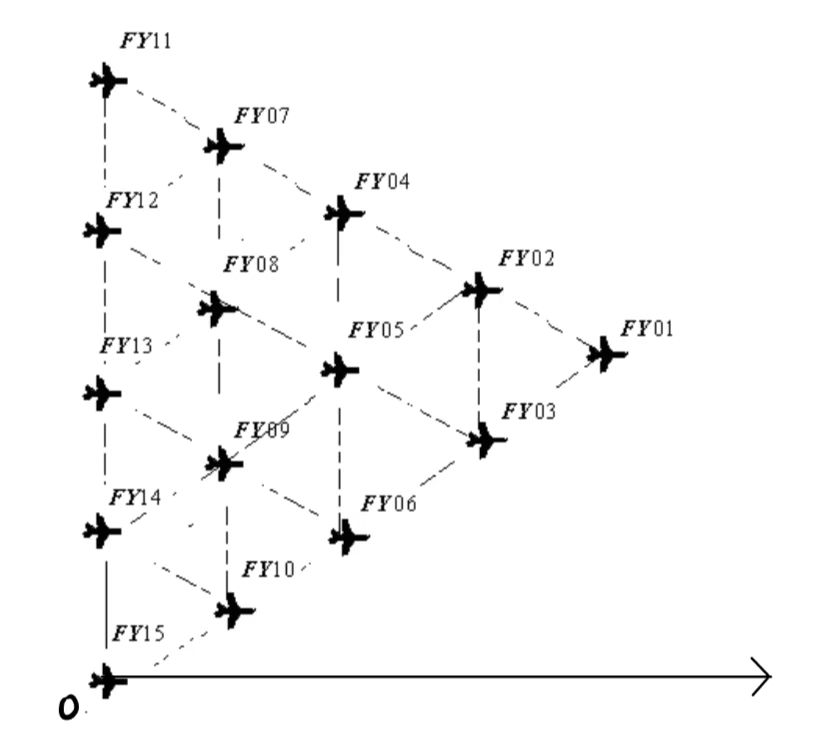
\includegraphics[scale=0.2]{pic/8.2.jpg}
		\caption*{图8}
	\end{figure}
		
	\par 建立坐标系后,参考问题一(1)中所建立的无人机无源定位模型,延续使用发射信号无人机与接受信号无人机的定义,即$\al_1,\al_2,\al_3$的定义。
	我们可以知道,无人机的定位必须依靠所接收到的$\al_1,\al_2,\al_3$角度信息,
	以及正确的距离关系,例如半径$r$的长度。
	在本题中,使用纯方位无源定位模型则也必须已知某无人机之间的长度关系,即使用纯方位无源定位模型时必须存在无偏的无人机。
	下面对。
	

	\subsubsection{锥形队列定位模型的建立}
	当发射信号的无人机位置无偏差时,通过之前所建立的直角坐标系,计算出定位模型的通解。
	每次选择编号为FY15的无人机和另外两架无人机遂行发射信号,其余无人机接受信号。
	假设发射信号的无人机位置无偏差且编号已知,对锥形队列的纯方位无源定位模型进行建立。

	\par 其中确定三架无偏的无人机选取另外一架无人机可能会出现的情况如下:

	\begin{figure}[htbp]
		\centering
		\subfigure{
			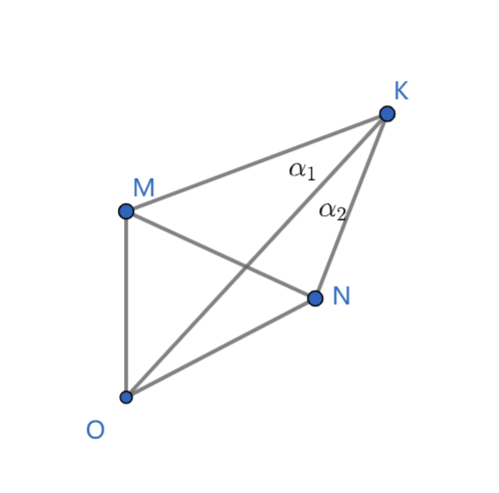
\includegraphics[scale=0.4]{pic/2.1.png}
		}
		\hspace{0.1in}
		\subfigure{
			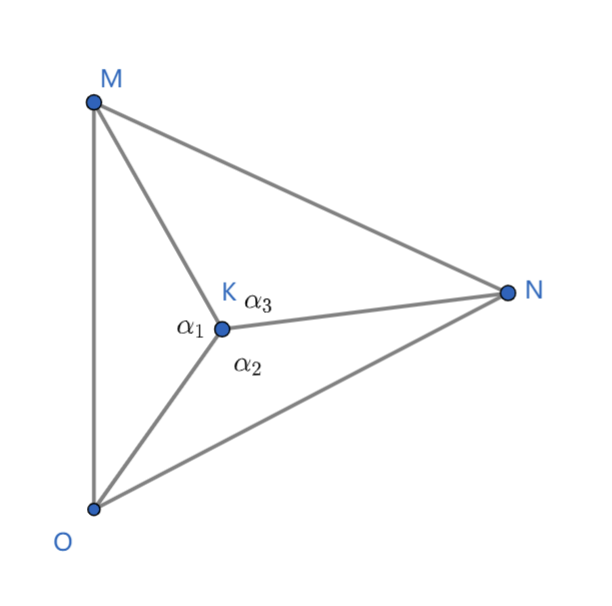
\includegraphics[scale=0.33]{pic/2.2.png}        
		}
		\hspace{0.1in}
		\subfigure{
			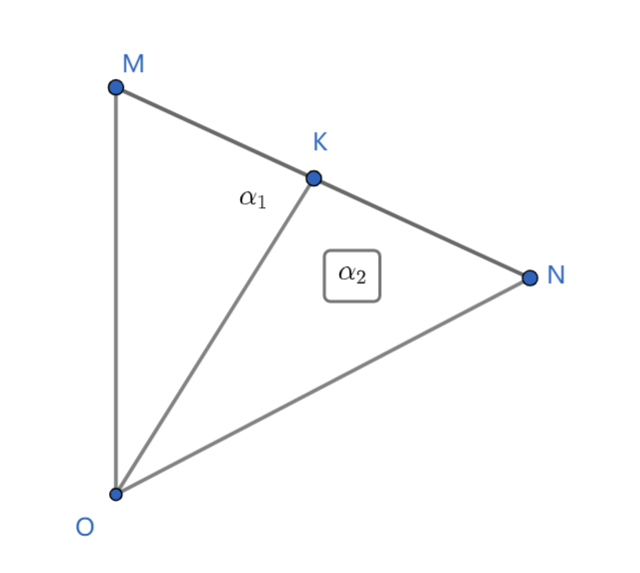
\includegraphics[scale=0.33]{pic/2.3.png}        
		}
		\hspace{0.1in}
		\subfigure{
			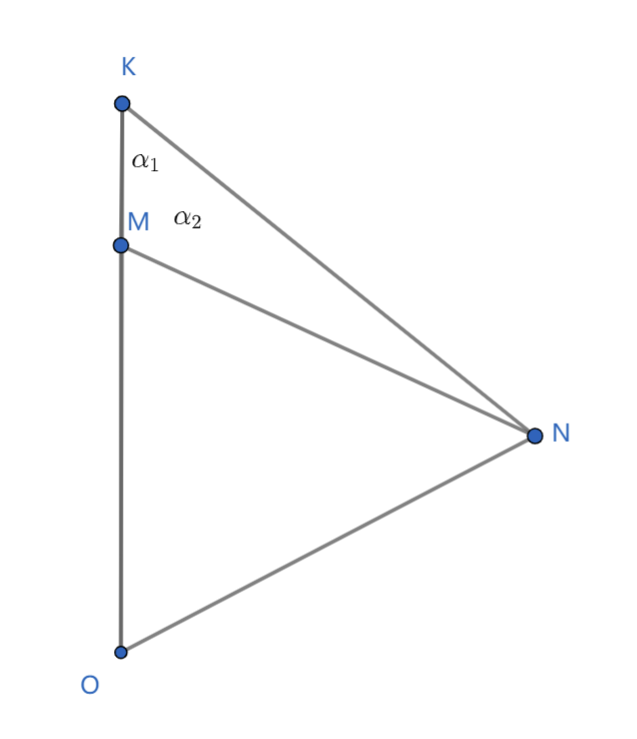
\includegraphics[scale=0.3]{pic/2.4.png}        
		}
		\caption*{图9}
	\end{figure}

	图中的O为坐标原点也就是FY15,M点与N点表示发射信号的无偏无人机,K点表示接受信号的无人机。
	当前的目标即是求解K点的相关坐标信息,
	利用三角函数的相关定理,就可以通过解三角形的方式求解。
	解出的前两个情况结果为 

\begin{equation}
	\begin{aligned}
		&\tan\angle ONK =\frac{OM \cdot \sin(2\al_1 + \angle MON)\cdot \sin\al_2}{ON\cdot \sin\al_1+OM \cdot \sin\al_2\cdot \sin(\al_1+\al_2+\angle MON)}\\
		&OK = \frac{ON}{\sin\al_2} \cdot  \cos\angle ONK 
	\end{aligned}
\end{equation}
	其中因为O,M,N的位置处于理想位置,则可以根据无人机的编号计算出OM,ON的长度以及角度$\angle MON$。
	 
	\par此外,当接收机K与OM共线时,如第三第四种情况,则需要分更细的情况进行讨论。
	求解出的结果如下
	
\begin{equation}
	\begin{aligned}
		OK=\frac{OM}{\sin\al_2}\cdot \sin(\al_2+\frac{\pi}{3})\;\;\mbox{或}\;\;\frac{OM}{\sin\al_1}\cdot \sin(\al_1+\frac{\pi}{3})
	\end{aligned}
\end{equation}

	\par
	其中K的相应角坐标与M的角坐标相同。
	$\al_1$与$\al_2$的选取是根据K与OM的相对位置而决定,当K处于OM内部时选取$\al_1$,处于外部时选取$\al_2$。
	分析可知当K与ON共线时则类似。

	\par当接收机K与MN共线时,求解出的结果为

\begin{equation}
	\begin{aligned}
		&\tan \angle ONK = -\frac{OM\cdot \sin(2\al_1 + \angle MON) \cdot \sin\al_2}{ON\cdot \sin\al_1 + OM\sin\al_2 \cdot \cos(\al_1 + \al_2+\angle MON)}\\
		&OK = \frac{ON}{\sin\al_2 }\cdot \sin \angle ONK
	\end{aligned}
\end{equation}

	至此则接受机的极坐标可以通过$\al_1,\al_2$求出,则锥形编队的无源定位模型建立完成。

	\subsubsection{锥形队列完备的定位选取}
	
	\par接下来需要求出除让FY15发射信号外,还需多少架无人机发射信号才能保证对其余的所有无人机进行定位。
	首先,接收机获得的$\al_1,\al_2$信息若其中一个为0或$\pi$或同时为0或$\pi$则表示接受机K与OM,ON共线,此时可以代入共线情况(5)方程组下求解。
	若角度信息$\al_1,\al_2$都不等于0或$\pi$,则可归类为不共线情况(4)号方程组下,对K的位置进行求解。

	现在我们考虑在(4)方程组下,当$\al_1,\al_2$都不为0或$\pi$时,有无可能存在无解的情况。

	要证明无解存在,即证明
	\begin{align*}
		ON\cdot \sin\al_1+OM \cdot \sin\al_2\cdot \cos(\al_1+\al_2+\angle MON)=0\;\;\;\mbox{存在。}
	\end{align*}

	因无法通过分析代数的方式判断该等式能否成立,故考虑采用大量数值逼近的手段判断该方程的解$(\al_1,\;\al_2)$能否成立。
	其中$\angle MON$可以确定为有限种情况,所以将ON,OM和$\al_1,\al_2$以足够小的步长进行整个范围的遍历,查看0解的存在性,即可判断能否使用三架无人机实现其余无人机的定位。
	经过分析可以知道,$\sin\al_1$与$\sin\al_2$是同号的,因为接收信号无人机处于等边三角形的内部,对于任意发射信号无人机的组合,
	故无论其为锐角或钝角,它的$\sin$已知为非负,该表述一直是正确可证的。
	另外,由三角形的相关公理,$\cos(\al_1+\al_2+\angle MON)$也一定处于$(0,\;2\pi)$之间。
	所以$\tan \angle ONK$中的分母不存在等于0的情况,即该tan值存在。
	
	经过程序运行与分析,在锥形编队中,仅需3架无人机即可实现其余无人机的定位。

	\subsubsection{锥形队列无人机位置调整方案}
	上文中证明了在无人机锥形编队下,加上原点无人机一共3架即可对其余的无人机位置进行定位,从而实现调整。

	因与问题一(3)类似,无人机编队的最终状态已知,则需要将当前无人机编队状态向最终状态调整。
	在假设中包括原点的三架无人机处在正确位置上,此时同样可以仅考虑一个无人机点的位置,从而在计算出其余无人机的位置,并使用直接调整的方式将无人机沿直线调整到理想位置上。
	即可同样仿照问题一(3)中的非线性优化问题,可以列出目标方程,
	\begin{align*}
		\min  \;\;\;\; d=\sm (p_i-p_i')
	\end{align*}

	并可以根据几何关系以及最后的理想编队位置找出相对应的限制条件,即为由已知的三个无偏点生成的特定$\d\t$准许范围,且每一个无人机对应以个$\d\t_i$。
	并以此方程组组成矩阵$A$,最后利用问题一(3)的\\
	MATLAB最优化算法求解出答案。
	解出的$\d\t_i,\d d$即为最后每一个无人机所要移动的角度与距离,最后使每一个无人机沿直线移动到计算出的位置上,
	此时就是该调整方案的最优解,使所有无人机总移动距离最短的调整方案。

\vspace{1em}
\section{模型优缺点分析}
	在问题一中所使用的纯方位无源定位模型实际上是一个利用角度信息定位的模型,每次通过3架无人机对另外一架无人机发射信号,从而计算出位置未知的无人机的相对位置。
	在建立了定位模型后,发现该模型存在一定的优势与劣势。

	\subsection{模型优势}
	纯方位无源定位模型可以仅根据不同无人机之间发射信号的角度信息,来实现无人机的定位,可以应用于实际中无人机之间的定位系统。
	对比其他依赖于坐标系距离的定位系统,无源定位模型所需的参数较少,且参数的获得较易。如可直接从接收信号的方向获取$\al_1,al_2$参数。
	另一方面,该定位模型的速度较快,仅涉及到简单的代数运算。

	\subsection{模型劣势}
	在问题的求解中,可以明显地感受到所有的定位都必需存在一定数量的位置无偏的无人机进行信号发射。
	因此当所有无人机的位置都有偏差时,或仅有1或2架无人机位置无偏时,则该模型无法对其余无人机进行定位。
	又或者仅对3架无人机所组成的编队进行位置调整,则无法获得足够的角度信息参数,定位无法实现。
	
\begin{thebibliography}{9} %参考文献
		\bibitem{bib:one}王元昊,曾红,数学基本问题的MATLAB解法. 北京:化学工业出版社,2019.8
		\bibitem{bib:two}吴建国,汪名杰,李虎军,数学建模案例精编. 北京:中国水利书店出版社,2005	
\end{thebibliography}
	
	\newpage
	\section{附录}

	问题一(3)的最优化求解代码如下(见支撑材料文件夹:问题一(3)的求解 pb13opt.m)
	\begin{lstlisting}
	clear,clc;
	format long
	syms dt1 dt2 dt3 dt4 dt5 dt6 dt7 dt8 dt9
	
	dt=sym([dt1,dt2,dt3,dt4,dt5,dt6,dt7,dt8,dt9]);
	tt=sym([0, 40.10, 80.21, 119.75, 159.86, 199.96, 240.07, 280.17, 320.28]);
	ro=sym([100, 98, 112, 105, 98, 112, 105, 98, 112]);
	ta=sym(tt/180*pi);
	tb=double(ta);
	A=zeros(9,9);
	B=zeros(9,1);
	
	dis=sym([]);
	r=sym(100.0);
	c=sym([]);
	init=zeros(1,9);

	for i=1:9
		dis(i)=(r^2+ro(i)^2-2*ro(i)*r*cos(dt(i)))^(1/2);
		
	end
	subj=sum(dis);

	for i=2:9
		c(i)=(dt(i-1)-dt(i)-((tt(i)-tt(i-1))+40)*180/pi);
		A(i,i-1)=1;
		A(i,i)=-1;
		B(i,1)=ta(i)-ta(i-1)-40/180*pi;
	end
	A(1,1)=-1;
	A(1,9)=1;
	B(1)=ta(1)-ta(9)+2*pi-40/180*pi;
	c(1)=dt(9)-dt(1)-((360-tt(9))+40)/180*pi;
	c=reshape(c,9,1);
	subj=sum(dis);
	[dt,fval]=fmincon(@fun1,init,[],[],A,B);
	dtp=dt/pi*180;
	% dt/pi*360
	% dt1,dt2,dt3,dt4,dt5,dt6,dt7,dt8,dt9
	\end{lstlisting}

	\newpage
	问题二的相关证明代码如下(见支撑材料文件 searchbypoint.m)
	\begin{lstlisting}
		point=[100*sqrt(3) 100;75*sqrt(3) 125;75*sqrt(3) 75;50*sqrt(3) 150;50*sqrt(3) 100;50*sqrt(3) 50;
		25*sqrt(3) 175;25*sqrt(3) 125;25*sqrt(3) 75;25*sqrt(3) 25;0 200;0 150;0 100;0 50];
		xk=point(:,1);				%xk表示的是发射信号的观测机无偏的横坐标
		yk=point(:,2);				%yk表示的是发射信号的观测机无偏的纵坐标
		a1star=-500;				%便于查看下文的 a1star值变化
		a2star=-500;
									%对于在长为100*sqrt(3)宽为200的长方形当中
			for i=1:14 				%选取M点
				for j=1:14			%选取N点
					if i~=j
						for x=0:0.1:174
							for y=0:0.05:100
								mom=acos((xk(i)*yk(j)+xk(j)*yk(i))/(sqrt(xk(i)^2+yk(i)^2)*sqrt(xk(j)^2+yk(j)^2)));
								a1=acos(((xk(i)-x)*(-x)+(yk(i)-y)*(-y))/(sqrt((xk(i)-x)^2+(yk(i)-y)^2)+(x^2+y^2)));
								a2=acos(((xk(j)-x)*(-x)+(yk(j)-y)*(-y))/(sqrt((xk(j)-x)^2+(yk(j)-y)^2)+(x^2+y^2)));
								if sqrt(xk(j)^2+yk(j)^2)*sin(a1)+sqrt(xk(i)^2+yk(i)^2)*sin(a2)*cos(a1+a2+mom)==0
									a1star=180*a1/pi;
									a2star=180*a2/pi;
								end
							end
						end    
					end
				end
			end
		\end{lstlisting}

	模型建立及求解见支撑材料 相关求解1、2。
\end{document}
